%%=========================================
\section[Eksperimenter \& Resultater]{Eksperimenter \& Resultater}
%%=========================================
\subsection{Evalueringsstrategier}
{\color{red}Hvordan kan eksperimentene evalueres?}

\subsection{Eksperimentsutførelse}
{\color{red}Hvordan ble eksperimentet utført?}

\subsubsection*{Gestegjenkjennelse gjennom fotodioder}
{\color{red}Hvordan ble eksperimentet utført?}
{\color{red}Dette avsnittet må kanskje skrives ut mye mer for å forklare stegvis alt som er gjort?}

Dette kapittelet har følgende bidrag:
\begin{itemize}
\item Jeg argumenterer for at en gestesensor i form av enkle fotodioder er et tilstrekkelig medium for enkel brukerinteraksjon (\ref{ch:2.minide}).
\item Jeg viser at maskinlæring kan benyttes for å lære et system å forstå enkle gester og viser at dette er et alternativ til å eksplisitt programmere forståelse (\ref{ch:2.resultater}).
\item Jeg viser at det holder med et titalls treningseksempler fra hver gest for å oppnå gode resultater med lineære modeller og at det med 50 eksempler oppnås en suksessrate på 96\% (\ref{ch:2.resultater}).
\end{itemize}

A large vocabulary of discrete abstract gestures is essentially a sign language. So I would think that everything that applies to voice also applies in this case.

A small set of spatially-directed gestures at a distance (point to objects on a screen and move them around — Oblong / Minority Report) is indirect manipulation, not direct manipulation. It's kind of just a fancy mouse. I personally think this is a step backwards, and my (brief) experience has not been positive.

Directly manipulating a virtual 3D representation (Iron Man, if I remember right?) would have the problem of not being able to feel what you're manipulating, which I suspect would really throw off your proprioceptive senses. My (brief) experiences trying to manipulate objects by Waving My Hands In The Air have not been positive, because my hands were rarely where I thought they were. (But maybe throw some haptics in there, either via gloves or remotely-induced, and you might have something.)

Ulempen med denne formen for gjenkjenning av gester er de samme som med sensorovervåking gjennom kameraer; følelsen av overvåking og sikker håndtering av sensitive data. Det finnes andre, mindre påtrengende metoder for å detektere gester. Infrarøde gestur-sensorer kan tilby en kontaktløs interaksjon med det smarte hjemmet\footnote{SparkFun RGB and Gesture Sensor. Denne brikken kan måle lys, farge, avstand og gester: https://www.sparkfun.com/products/12787, hentet des 2014.}. Sensoren sender ut infrarøde signaler og mottar refleksjonen fra brukerens hånd. Mikrokontrolleren må så tolke disse verdiene til en gest. Systemet kan dermed trenes med teknikker fra maskinlæring til å klassifisere og tolke forskjellige gester til å forskjellige kommandoer. Det infrarøde signalet reflekteres effektivt kun ut til en avstand på noen titalls centimeter. Dette blir dermed en mye mindre påtrengende metode enn bruk av video. Et bruksområde for gester kan være å be om det neste steget i en oppskrift, uten å måtte trykke på en touch-skjerm mens hendene er tilskitnet med mat. Det kan også være aktuelt å kombinere gester med en annen interaksjonsform, som tale. Et multimodalt brukergrensesnitt kan forbedre systemets nøyaktighet i tolkningen av kommandoene og avklare usikkerhet og misforståelser.

{\color{red}PING: Maskinlæring kan benyttes for å gi enkle sensorer en svært god forståelse av gester.}
Dette avsnittet presenterer hovedidéen for dette kapitellet. 
Dersom man ønsker å tilby styringsmuligheter på en eller flere vegger i et hus kan enkle gestesensorer benyttes i steden for et panel av knapper og dimmere. Selve sensoren er på størrelse med et knappenålshode og vi kan dermed forestille oss at designere kan komme opp med produktimplementasjoner som enten forsvinner inn i hjemmiljøet eller synes tydelig, men er praktisk og estetisk veldesignet. Sensoren merker at en hånd eller et annet objekt befinner seg foran den ved å sende ut et svakt infrarødt signal som reflekteres og detekteres dersom signalet er sterkt nok når det returnerer. Dette vil bare skje dersom objektet er opptil 20 cm unna sensoren. Dette betyr at gester kun forstås dersom de utføres rett foran sensoren. I motsetning til forståelse av gester gjennom bruk av kameraer er dette altså en langt mindre påtrengende måte å "lytte" etter innspill fra brukerne. Brukere kan være sikre på at de hverken overvåkes eller at personvernet deres på noen måte brytes. En slik gestesensor fungerer rett og slett kun som en multifunksjonell knapp.

\begin{wrapfigure}{r}{0.4\textwidth}
    \vspace{-20pt}
  \begin{center}
    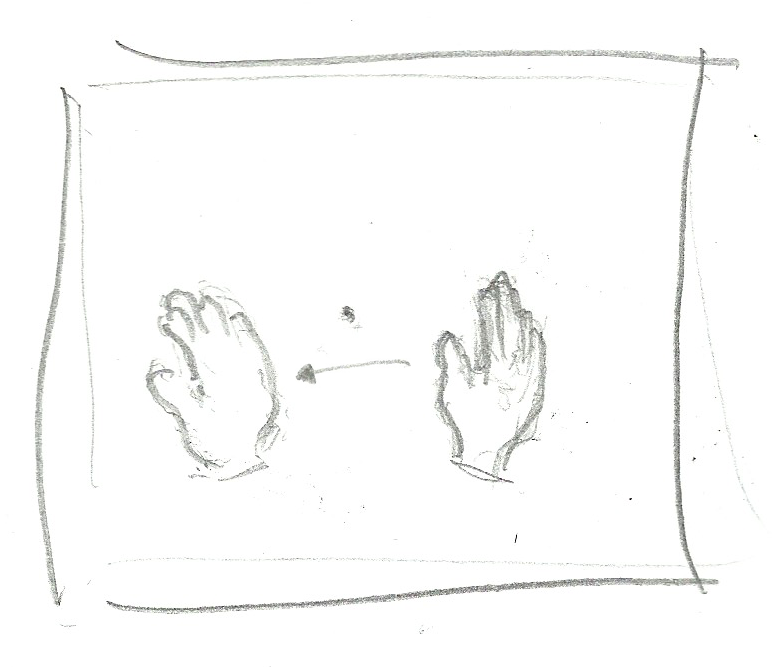
\includegraphics[width=0.35\textwidth]{fig/swipe-l-r}
  \end{center}
  \vspace{-20pt}
  \caption{Illustrasjon av en typisk gest.}
  \label{fig:gest}
  \vspace{-7pt}
\end{wrapfigure}

Figur \ref{fig:gest} viser en typisk gest der brukeren sveiper hånda foran sensoren som befinner seg på veggen. Vi kan forestille oss at denne sveipende bevegelsen foran denne sensoren betyr å skru av lyset i rommet sensoren befinner seg i. Men kanskje gesten betyr å skru på radioen, lukke gardinene eller starte kaffemaskinen. Det er ingen begrensning på hva en enkelt gest aktiverer i form av funksjonalitet.

Når en gest utføres må enten rådataene fra sensoren eller en forståelse av dataene sendes til en maskin som har ansvaret for å styre apparatene i hjemmet. Sensoren må være knyttet til en mikrokontroller eller tilsvarende som har ansvaret for å sende dataene videre. Dette kan enten være gjennom kabel eller trådløst. Det er mulig å programmere en mikrokontroller til å skille mellom sensordataene og forstå seks ulike gester {\color{red} ref}. Dette er i seg selv bra og betyr at en enkelt sensor kan fungere som en multifunksjonell knapp med minimum seks forskjellige kommandoer. Hvis man også utnytter at kombinasjonen av flere gester etter hverandre kan bety egne kommandoer er styringsmulighetene mange. Det finnes et alternativ til å programmere inn hva de ulike dataene skal tolkes som. Alternativet er å sende rådataene til en kraftigere maskin som kan benytte den spennende teknikken kjent som maskinlæring til å forstå enda flere ulike gester, med god sannsynlighet for suksess.


Når Python-scriptet{\color{red} ref process-data.py} kjøres på datamaskinen åpnes tilkoblingen til å lytte på den riktige serielle porten. Porten åpnes i noen sekunder og ber om at en gest utføres.Jeg gjennomførte 50 utførelser av hver av de 10 gestene\ref{fig:gester}, for totalt 500 datapunkter. Dataene fra hver gest ble lagret i individuelle filer i kommaseparert format. Med dataene for hver gest lagret i forskjellige filer kan disse kombineres slik man ønsker for å trene systemet til å skille mellom 2,3, eller opp til 10 gester. 

Maskinlæring handler om å la maskinen lære fra data. Dette kan enten være et forsøk på å finne ukjente sammenhenger i dataene den mates med eller det kan være å lære seg sammenhenger mellom dataeksempler og etiketter/klasser. Det er dette sistnevnte scenariet vi er interessert i. Vi kan mate maskinen med data fra en gest og samtidig gi informasjon om at dataene maskinen akkurat fikk betyr "sveip til høyre". Dermed kan maskinen danne en kobling mellom dataene som kom inn da vi sveipet til høyre og etiketten "sveip til høyre". Med tilstrekkelig treningseksempler fra de ulike gestene skal maskinen kunne lære seg forskjellene mellom de ulike gestene. Dermed vil den være i stand til å gjette riktig på hvilken gest vi utfører ved en senere anledning. Prototypen jeg har utviklet er trent med 50 ulike dataeksempler på hver av de 10 ulike gestene.



\begin{figure}[h]
\begin{subfigure}{0.23\textwidth}
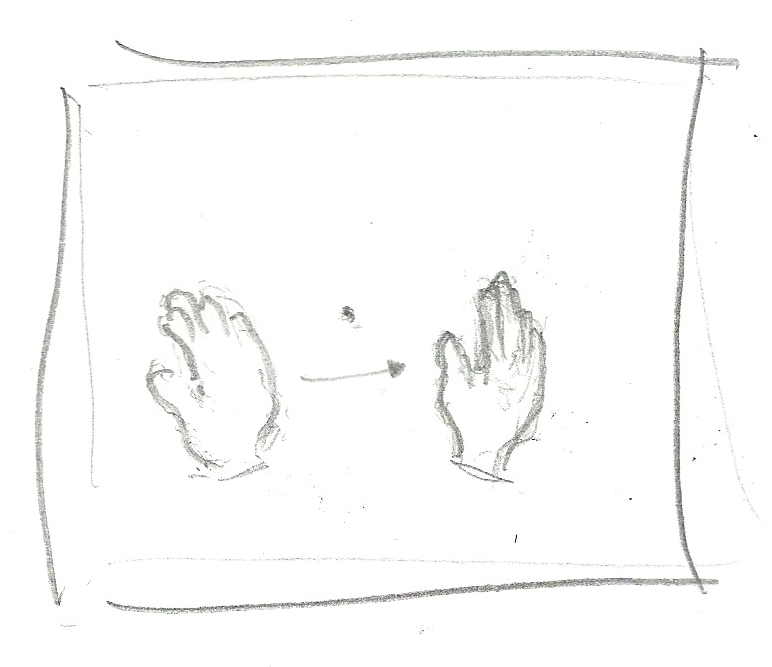
\includegraphics[width=3cm, height=3cm]{fig/swipe-r-l}
\caption{Sveip til høyre.}
\label{fig:sveip-}
\end{subfigure} 
\begin{subfigure}{0.23\textwidth}
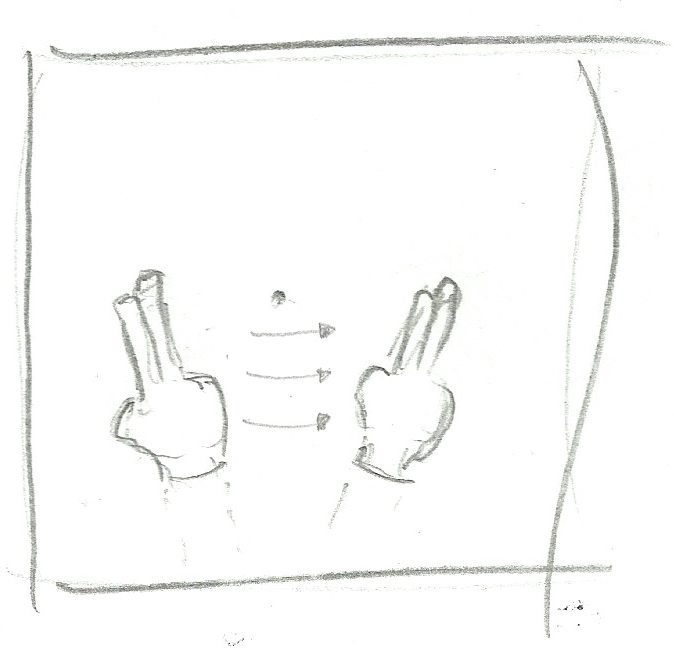
\includegraphics[width=3cm, height=3cm]{fig/flick-l-r} 
\caption{Flikk til høyre.}
\label{fig:flikk-h}
\end{subfigure}
\begin{subfigure}{0.23\textwidth}
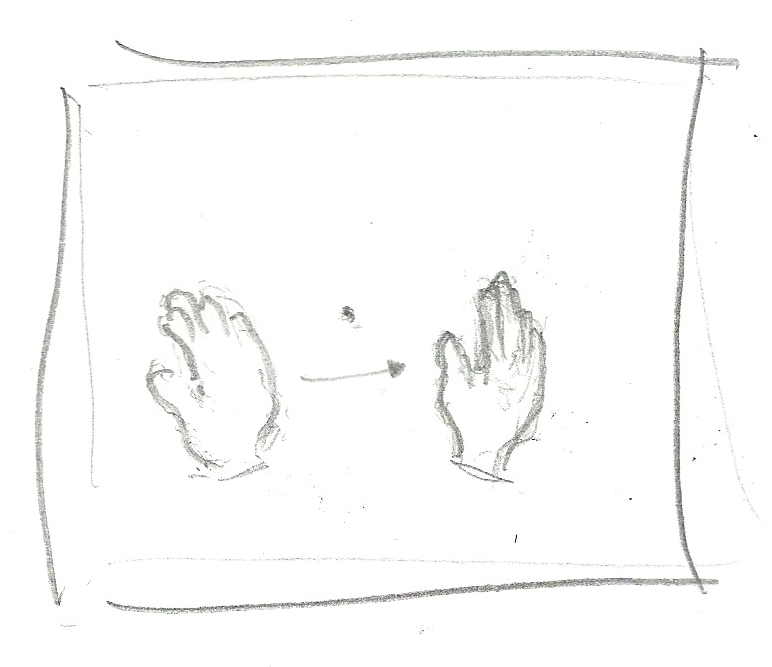
\includegraphics[width=3cm, height=3cm]{fig/swipe-r-l}
\caption{Sveip til venstre.}
\label{fig:sveip-v}
\end{subfigure} 
\begin{subfigure}{0.23\textwidth}
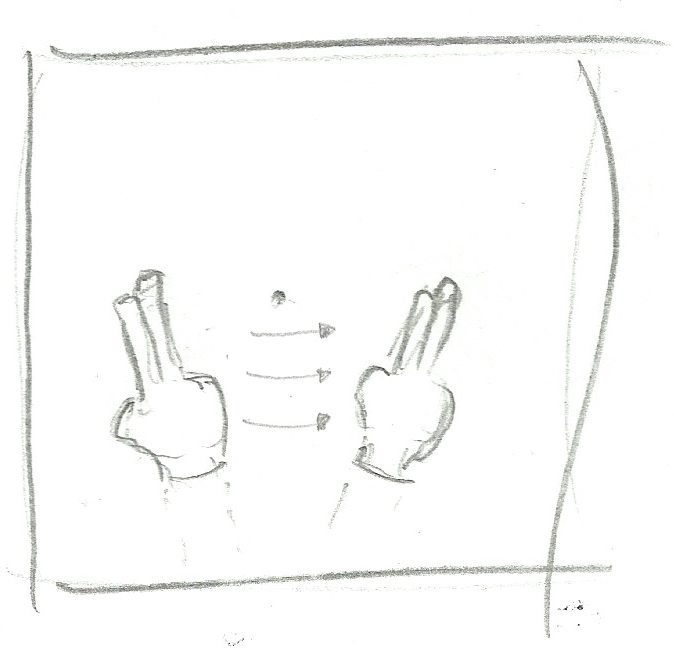
\includegraphics[width=3cm, height=3cm]{fig/flick-l-r}
\caption{Flikk til venstre.}
\label{fig:flikk-v}
\end{subfigure}
\begin{subfigure}{0.23\textwidth}
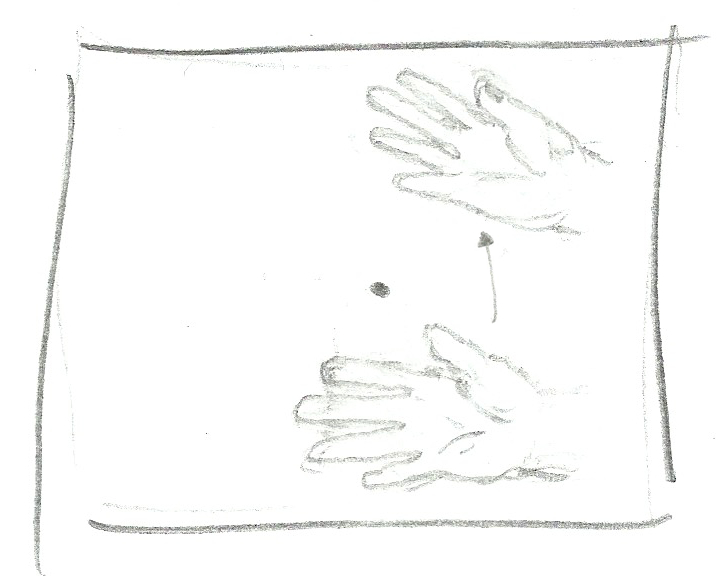
\includegraphics[width=3cm, height=3cm]{fig/swipe-d-u}
\caption{Sveip opp.}
\label{fig:sveip-opp}
\end{subfigure}
\begin{subfigure}{0.23\textwidth}
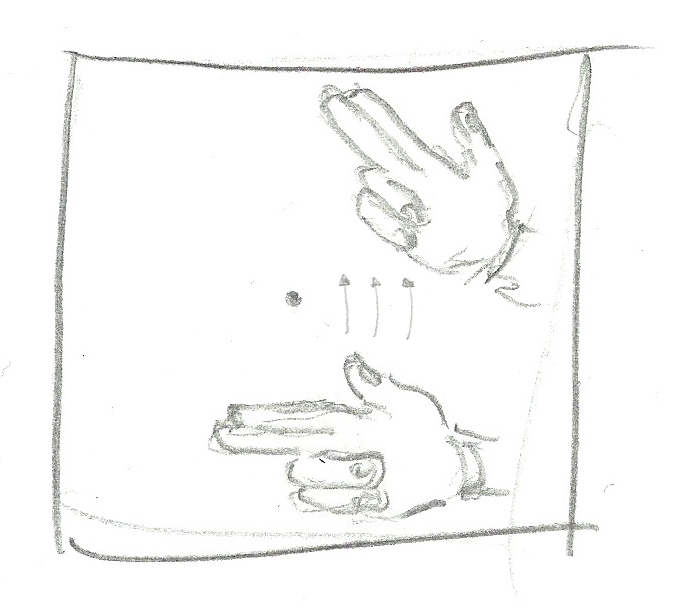
\includegraphics[width=3cm, height=3cm]{fig/flick-d-u}
\caption{Flikk opp.}
\label{fig:flikk-opp}
\end{subfigure}
\begin{subfigure}{0.23\textwidth}
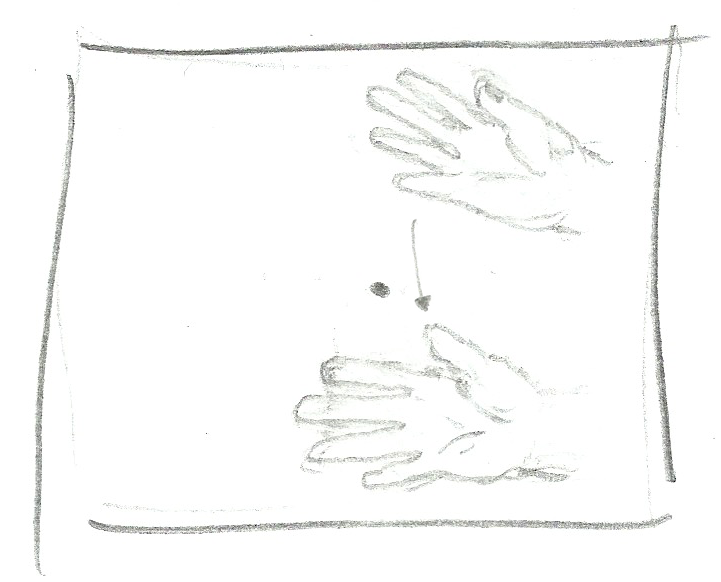
\includegraphics[width=3cm, height=3cm]{fig/swipe-u-d}
\caption{Sveip ned.}
\label{fig:sveip-ned}
\end{subfigure}
\begin{subfigure}{0.23\textwidth}
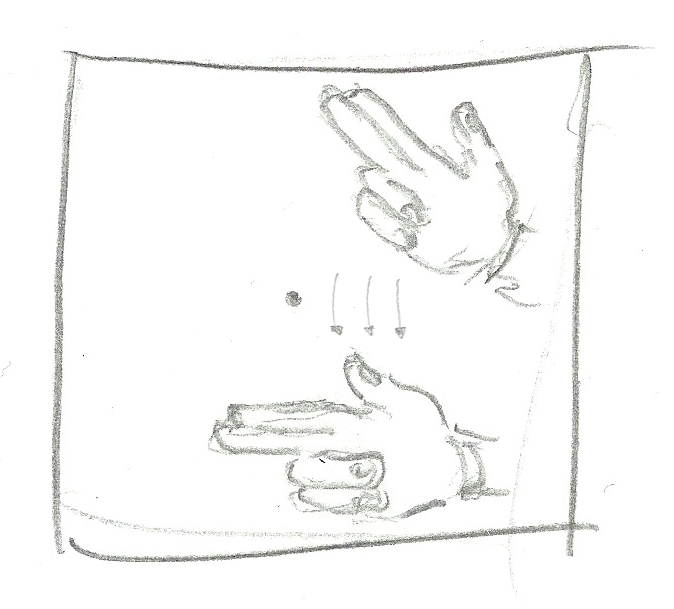
\includegraphics[width=3cm, height=3cm]{fig/flick-u-d}
\caption{Flikk ned.}
\label{fig:flikk-ned}
\end{subfigure}
\begin{subfigure}{0.25\textwidth}
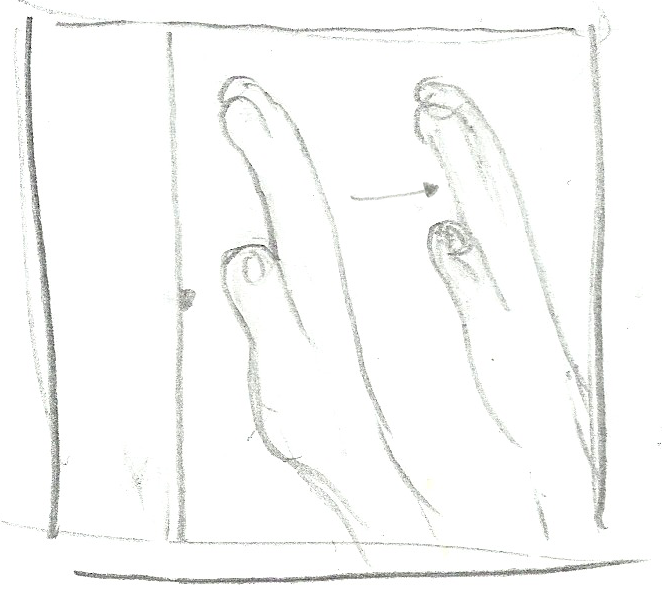
\includegraphics[width=3cm, height=3cm]{fig/near-far}
\caption{Nær - fjern.}
\label{fig:n-f}
\end{subfigure}
\begin{subfigure}{0.23\textwidth}
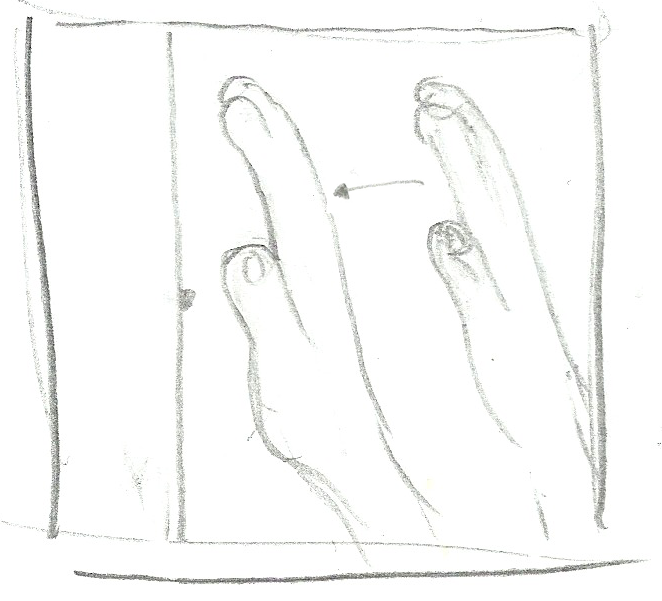
\includegraphics[width=3cm, height=3cm]{fig/far-near}
\caption{Fjern - nær.}
\label{fig:f-n}
\end{subfigure}
\caption{Illustrasjoner av de ulike gestene.}
\label{fig:gester}
\end{figure}

Python-scriptet {\color{red} ref learning.py} utfører maskinlæringen. Dataene blir lastet inn fra de aktuelle csv-filene og de aktuelle klassene opprettes. Man splitter så dataene i et treningssett og et testsett. Splittingen var 75\% til trening og 25\% til testing. Dette er et viktig steg i prosessen for å ikke spesialisere modellen til dataene. Dersom man trener på hele datasettet og tester på det samme settet er det en sjanse for at man har tilpasset modellen for mye til datasettet og ikke funnet den underliggende, generelle modellen. Hver modell blir trent og testet 100 ganger med et tilfeldig utgangspunkt hver gang, og sluttresultatet er et gjennomsnitt av disse.

\begin{figure}[h]
\centering
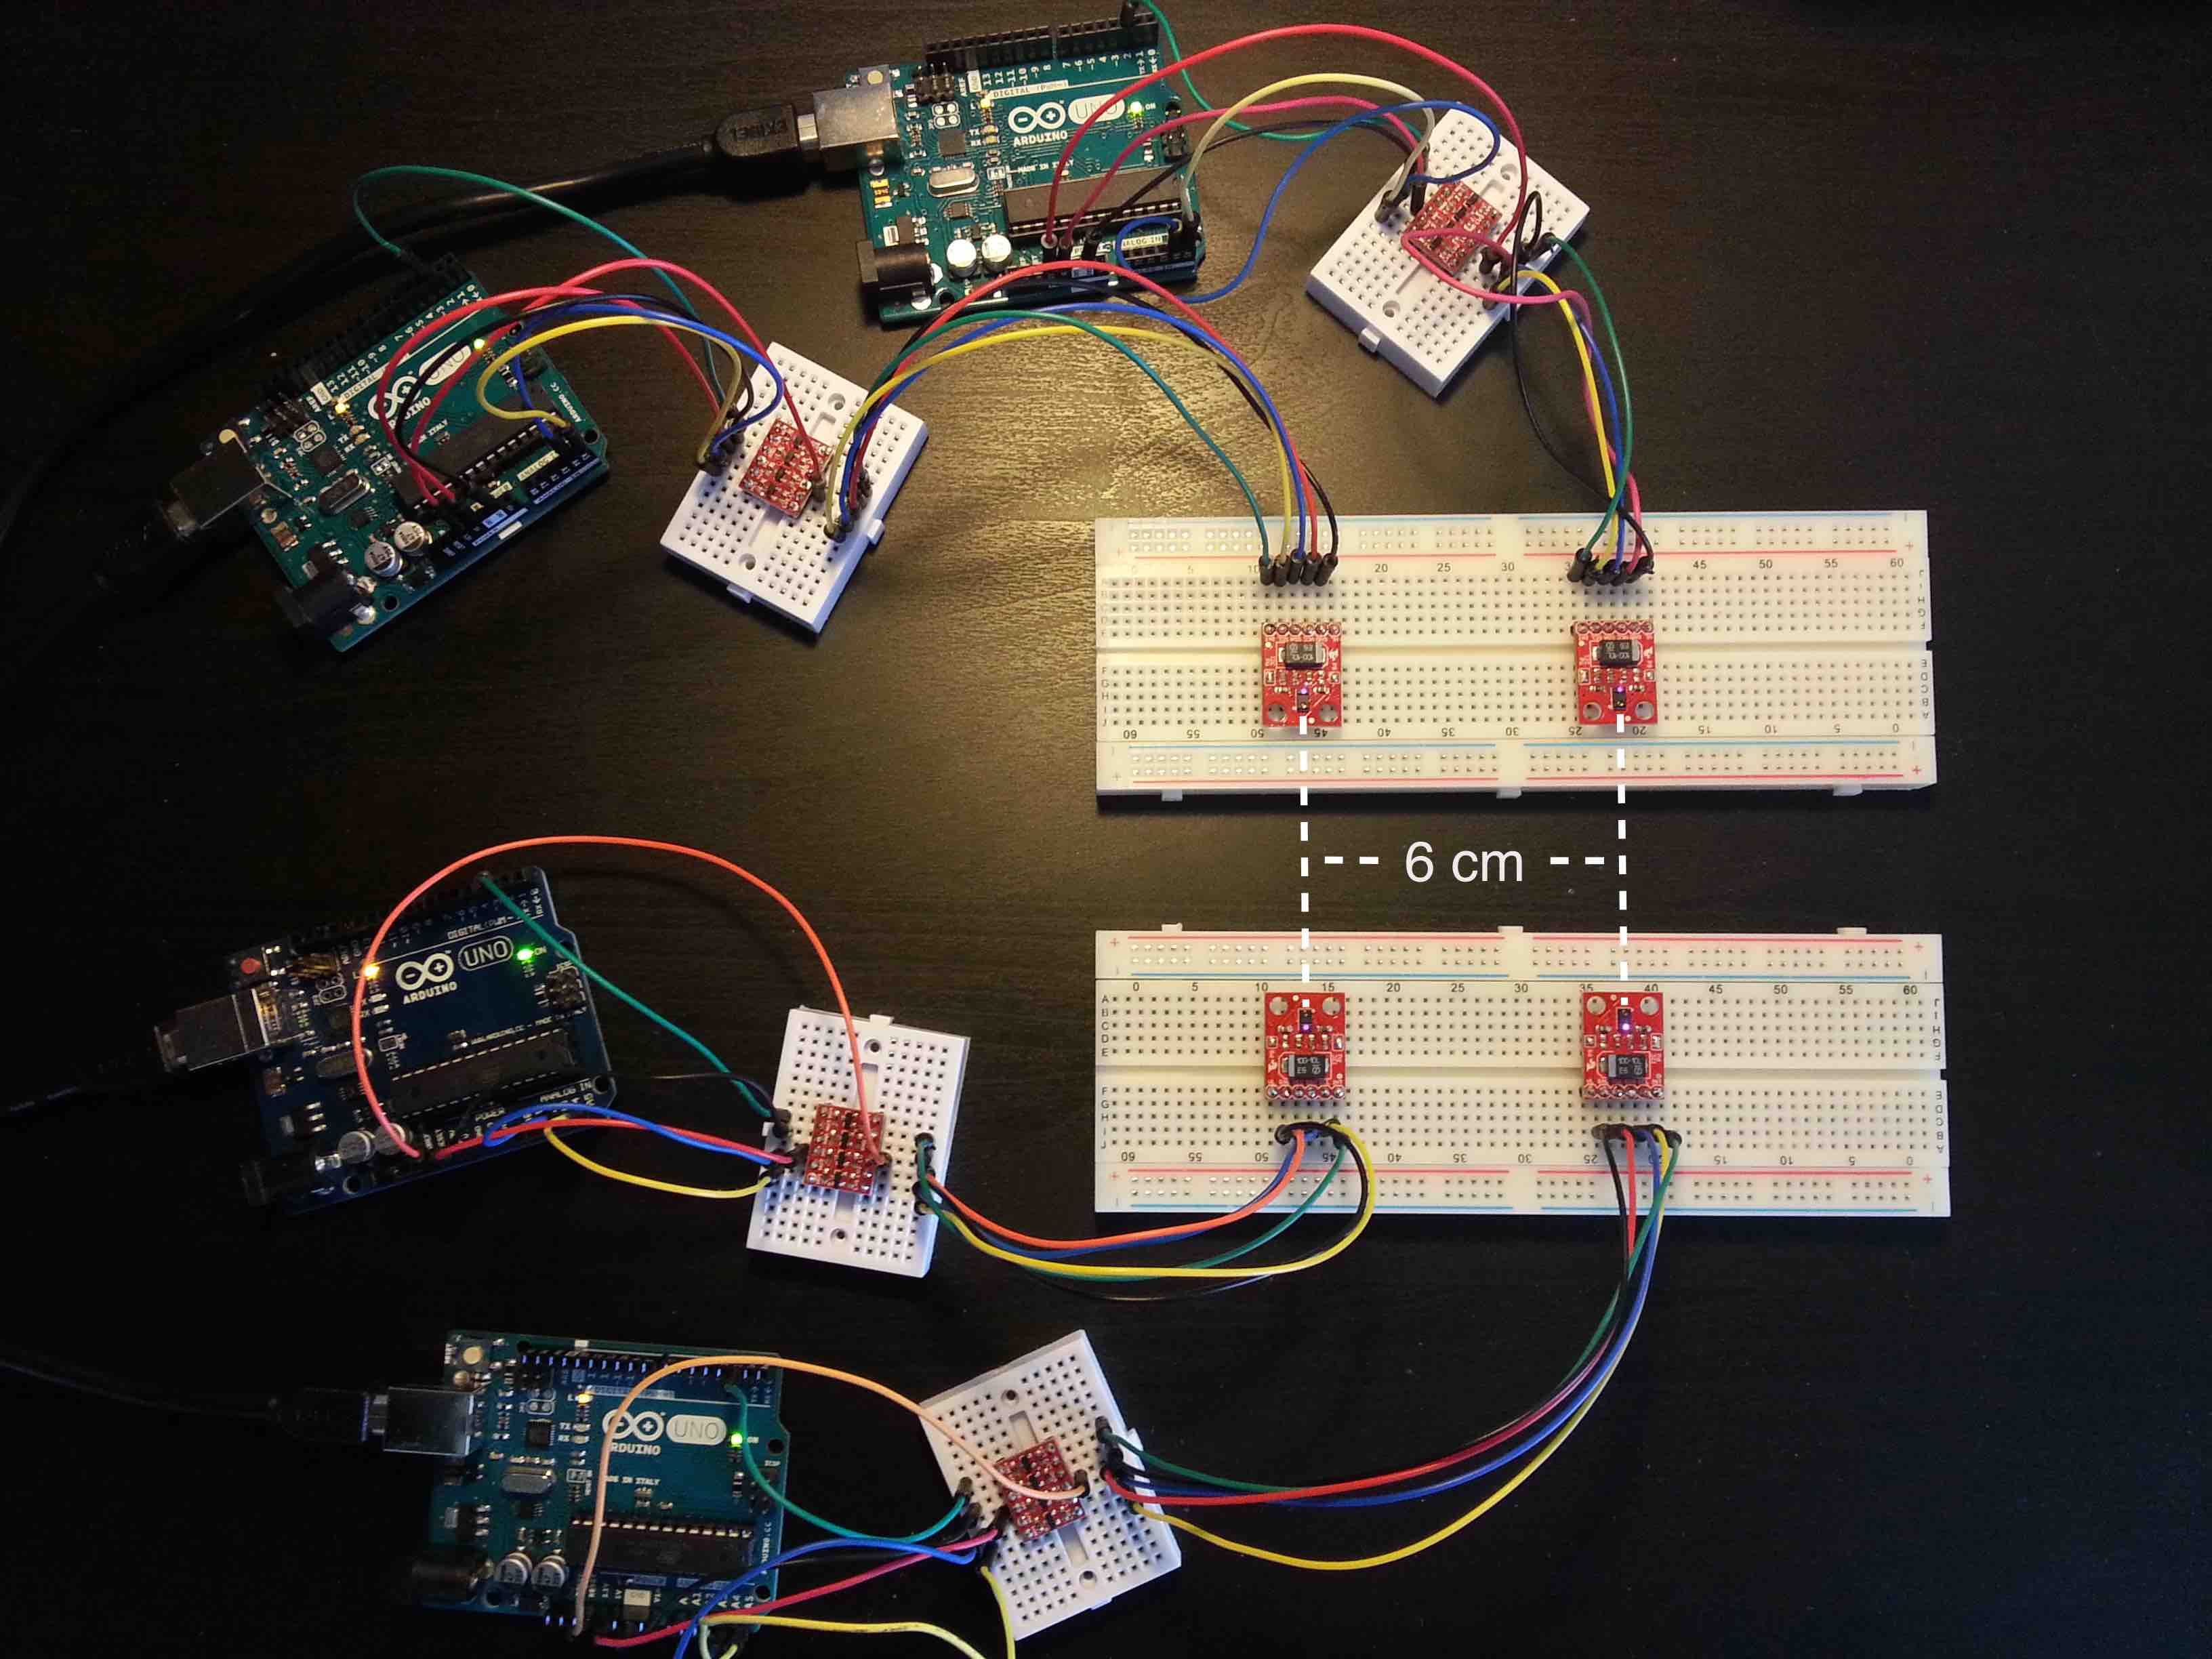
\includegraphics[width=15cm, height=12cm]{fig/foursensors}
\caption{Fire sensorer.}
\label{fig:four-sensors}
\end{figure}



\subsubsection{Multimodal interaksjon gjennom tale og gester}
{\color{red}Hvordan ble eksperimentet utført?}
lage ordbok

Det må etableres at kontinuerlig tale er et problem i henhold til personvern og responstid, gjennom logisk argumentasjon og empiriske bevis. Det samme gjelder for bruken av kommunikasjonsprogramvare i smarte hjem.

En annen, mer avansert, løsning er å benytte stemmegjenkjenning, der systemet forstår hvem som taler basert på talerens unike vokaltrakt. Dermed kan systemet programmeres til å kun godta kommandoer fra gjenkjente og klarerte brukere. Et annet alternativ er å tilby talegjenkjenning og syntesert tale bare i visse områder av hjemmet, som for eksempel på badet, der det er vanlig å tilbringe tid alene.

Mennesker i mellom kommuniserer i hovedsak med tale. Det er forsket mye på å få datamaskiner til å forstå og bruke denne naturlige kommunikasjonsformen og det er liten tvil om at det er en stor drøm for mange å kunne ha en kontinuerlig samtale med datamaskinen. 
På kjøkkenet hadde det også vært spennende å interagere gjennom tale mot systemet, for eksempel i forbindelse med bruk av en oppskrift. Det hadde også vært fordelaktig å ha naturlig kommunikasjon med systemet i sammenhenger der man jobber hjemmefra, enten profesjonelt eller med en hobby. Å ha et system som kan spørres om hjelp til enhver tid virker verdifullt.
Dette kapittelet har følgende bidrag:
\begin{itemize}
\item Argumenterer for at kombinasjonen av enkle gester og talekommandoer er en effektiv måte å interagere med det smarte hjemmet på {\color{red} fwd ref}.
\item Viser at talegjenkjenning over en begrenset mengde ord dekker funksjonaliteten vi ønsker å tilby gjennom tale og at det finnes åpne og tilgjengelige løsninger for å løse dette problemet.{\color{red} fwd ref}.
\item En implementasjon som håndterer multimodal input fra gestesensor og mikrofon. Denne benyttes for å simulerer bruken i et smart hjem ved å vise en dynamisk grafisk representasjon av inputdataene. Forskjellige anvendelser blir utforsket. {\color{red} fwd ref}.
\end{itemize}

Hva er en mer naturlig kommunikasjonsform enn tale? Generelt er det svært vanskelig å tenke seg andre former som kan beskrives som mer naturlige. Avhengig av hva som skal kommuniseres kan ulike tilnærminger være gode. Dersom man ønsker å skape noe gjennom manipulasjon blir tale raskt forbigått av en taktil kommunikasjonsform, som direkte kommunikasjon med hendene. Men når det gjelder å gi enkle kommandoer, å hente informasjon eller å kommunisere med andre mennesker kan tale fremstå som både den mest naturlige og effektive kommunikasjonsformen.

Drømmen om å kommunisere kontinuerlig med datamaskinen gjennom tale er tydelig gjennom både media og hvor penger til forskning plasseres. Denne oppgaven omhandler bruken av disse interaksjonsformene i konteksten av hjemmet. Så selv om tale kan være en interaksjonsform med stort potensiale i ulike domener må vi her spørre oss om å tilby tale som interaksjonsform er ønskelig i et hjem-scenario. 

{\color{red}PING: Kombinasjonen av enkle gester og begrenset tale er en aktuell og relativt enkelt implementerbar interaksjonsform for å styre det moderne hjemmet.}

Sure. Let's use voice for the things people use voice for — asking questions and issuing commands. But I'm personally interested in tools for creating and understanding.

Creating: I have a hard time imagining Monet saying to his canvas, "Give me some water lilies. Make 'em impressionistic." Or designing a building by telling all the walls where to go. Most artistic and engineering projects (at least, non-language-based ones) can't just be described. They exist in space, and we manipulate space with our hands.

Understanding: If you simply want information — "What's the price of AAPL over the last three years" — then an "oracle" like Wolfram Alpha is fine. But I believe that deep understanding requires active exploration, and I'm much more interested in explorable environments. Look at the interactive graphics in the Ladder of Abstraction essay, especially the later ones. You come to understand the system by pointing to things, adjusting things, moving yourself around the space of possibilities. I don't know how to point at something with my voice. I don't know how to skim across multiple dimensions with my voice.



%BBC http://www.bbc.com/news/technology-31296188
%CMUSphinx http://cmusphinx.sourceforge.net/2015/02/current-state-of-offline-speech-recognition-and-smarttv/

Problemene rundt Samsungs policy rundt talegjenkjenningsteknologien har skapt en del blest på internettet. Brukere har vist misnøye med at alt de sier i stua kan bli tatt opp og sendt til tredjeparter. 

Hva er statusen til talegjenkjenningsteknologi som ikke benytter kommunikasjon over internettet til kraftige servere på den andre siden?  

Talegjenkjenning på serveren har andre ulemper enn personvern. Det er for eksempel vanskelig å garantere en god responstid. Dersom det tar flere sekunder for dataene å nå serveren, bli prosessert og et resultat returneres kan nytteverdien til talegjenkjenning synke raskt. Umiddelbar respons er langt mer attraktivt.

Moderne telefoner, tv-er og andre enheter blir stadig kraftigere, men de er langt unna supercomputerene som for eksempel kjører Google's talegjenkjenning. Med flere prosessorkjerner vil ytelsen igjen øke i framtiden, men full bruk av disse trekker kraftig på batteriet.

Pocketsphinx er CMUSphinx-prosjektets talegjenkjenningsmotor designet for mobile enheter og andre alternative, ressursbegrensede plattformer. Pocketsphinx har et konfigurerbart vokabular så man kan skape modellene man trenger. Med god konfigurering kan Pocketsphinx gjenkjenne 10000 ord i reelltid med en feilrate på omtrent 20\%. Med midre vokabular kan presisjonen øke betraktelig og med under 100 ord er feilraten 3\%. Man kan også benytte et aktiveringsord slik at enheten kan lytte kontinuerlig gjennom dagen. Disse egenskapene gjør Pocketsphinx til et interessant valg når problemdomenet vårt tilsier at vi ønsker et system som gjenkjenner et titalls kommandoer i reelltid. Det er altså ikke nødvendig å knytte forståelsen opp mot internettet og sende taledataene ut i verden. Vi kan unngå problemene med personvern som Samsung og andre styrer med ved å holde all data lokalt. Vi ofrer en mer naturlig, kontinuerlig tale mot kommandoord, i bytte med en garantert bevarelse av personvernet.

Rejecting out of grammar utterances.

\subsubsection{Kombinasjoner}
{\color{red}Hvordan ble eksperimentet utført?}


Bruksområder i smarte hjem for de andre funksjonaliteten i sensorene.
PING: Data om farger, lysintensitet, avstand og en kombinasjon av flere gestesensorer utforskes for å finne nye interaksjonsideér.
Gester
Lysstyrke / Farger kontinuerlig
Lys interrupt
Nærhetsmåling kontinuerlig
Nærhetsinterrupt
Hva kan man få til dersom man har fire sensorer plassert i et kvadrat?

\begin{figure}[h]
\centering
\begin{subfigure}{0.23\textwidth}
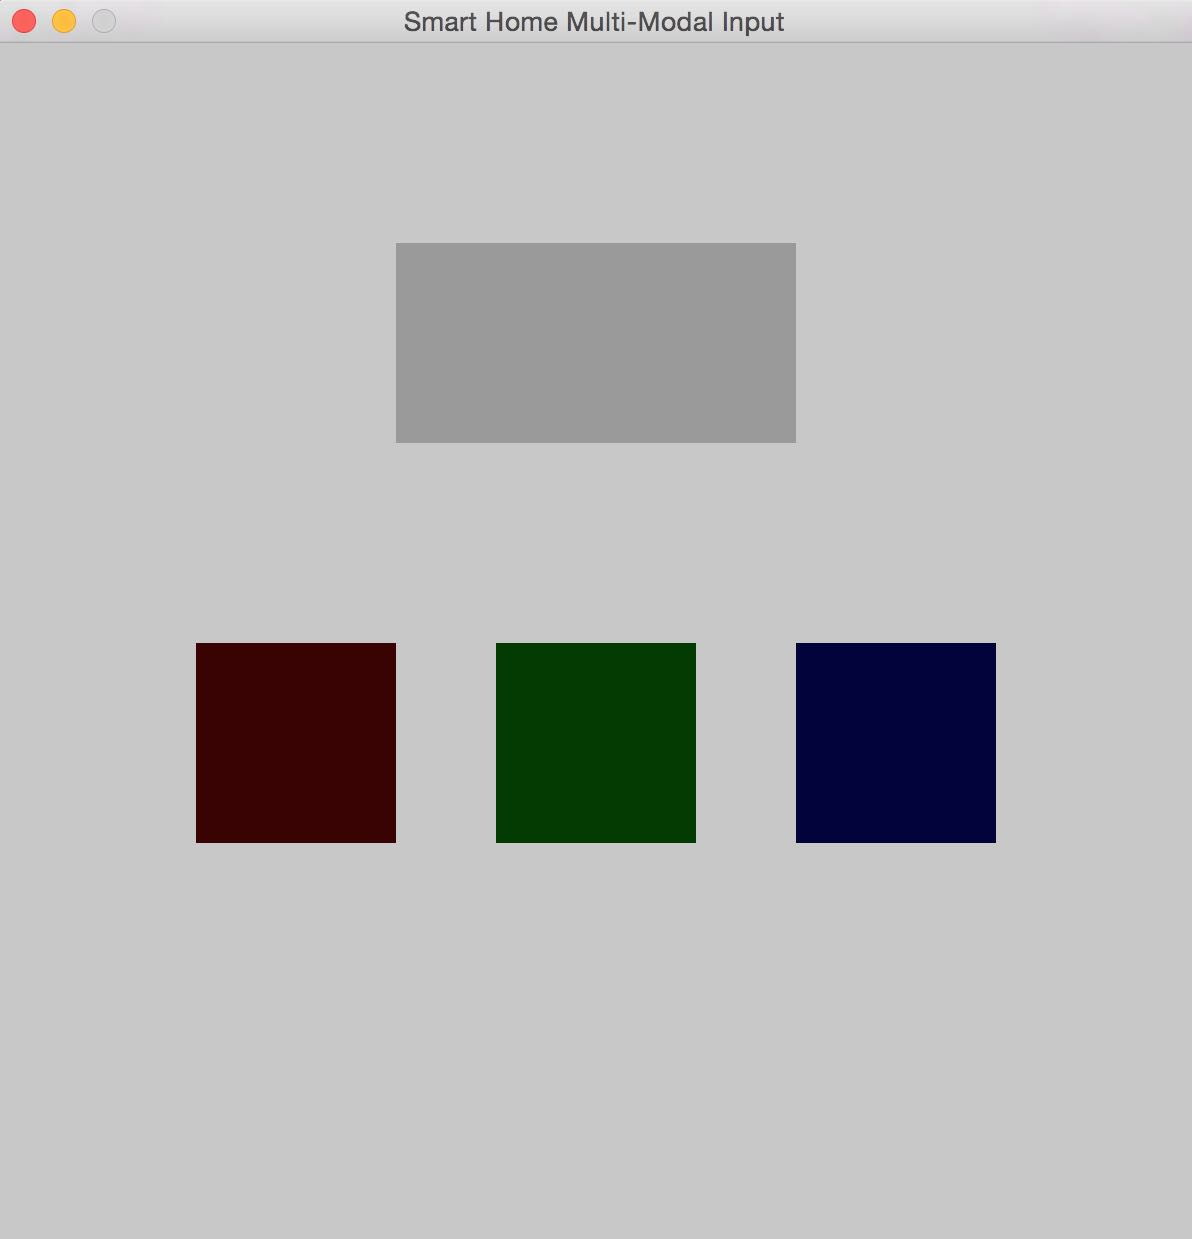
\includegraphics[width=3cm, height=3cm]{fig/color-1}
\caption{}
\label{fig:color-1}
\end{subfigure}
\begin{subfigure}{0.23\textwidth}
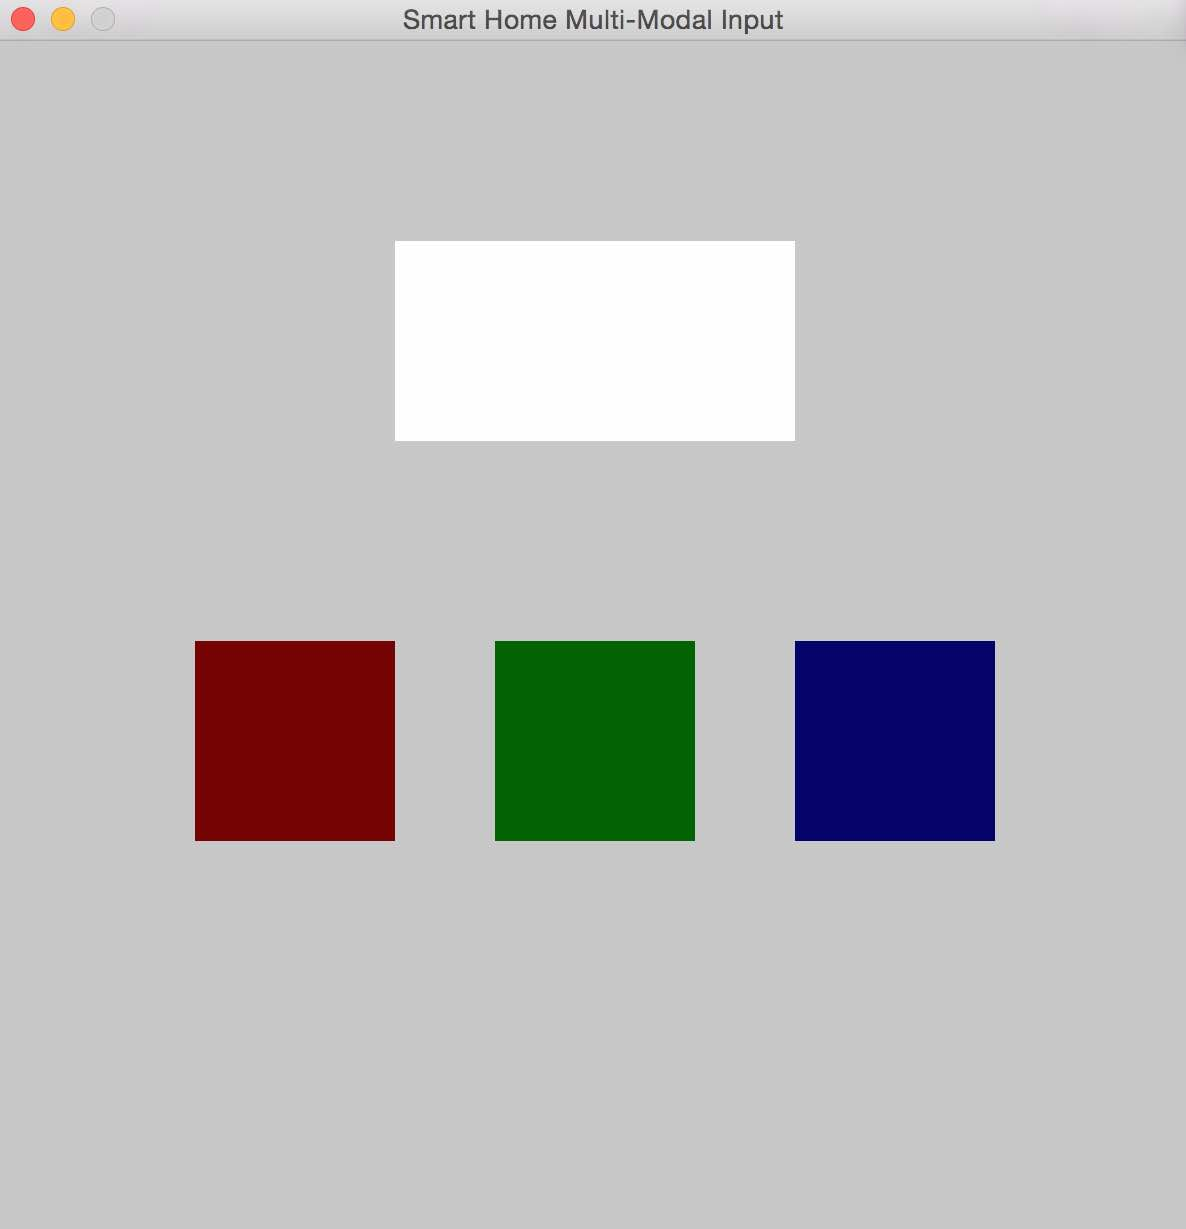
\includegraphics[width=3cm, height=3cm]{fig/color-2}
\caption{}
\label{fig:color-2}
\end{subfigure}
\begin{subfigure}{0.23\textwidth}
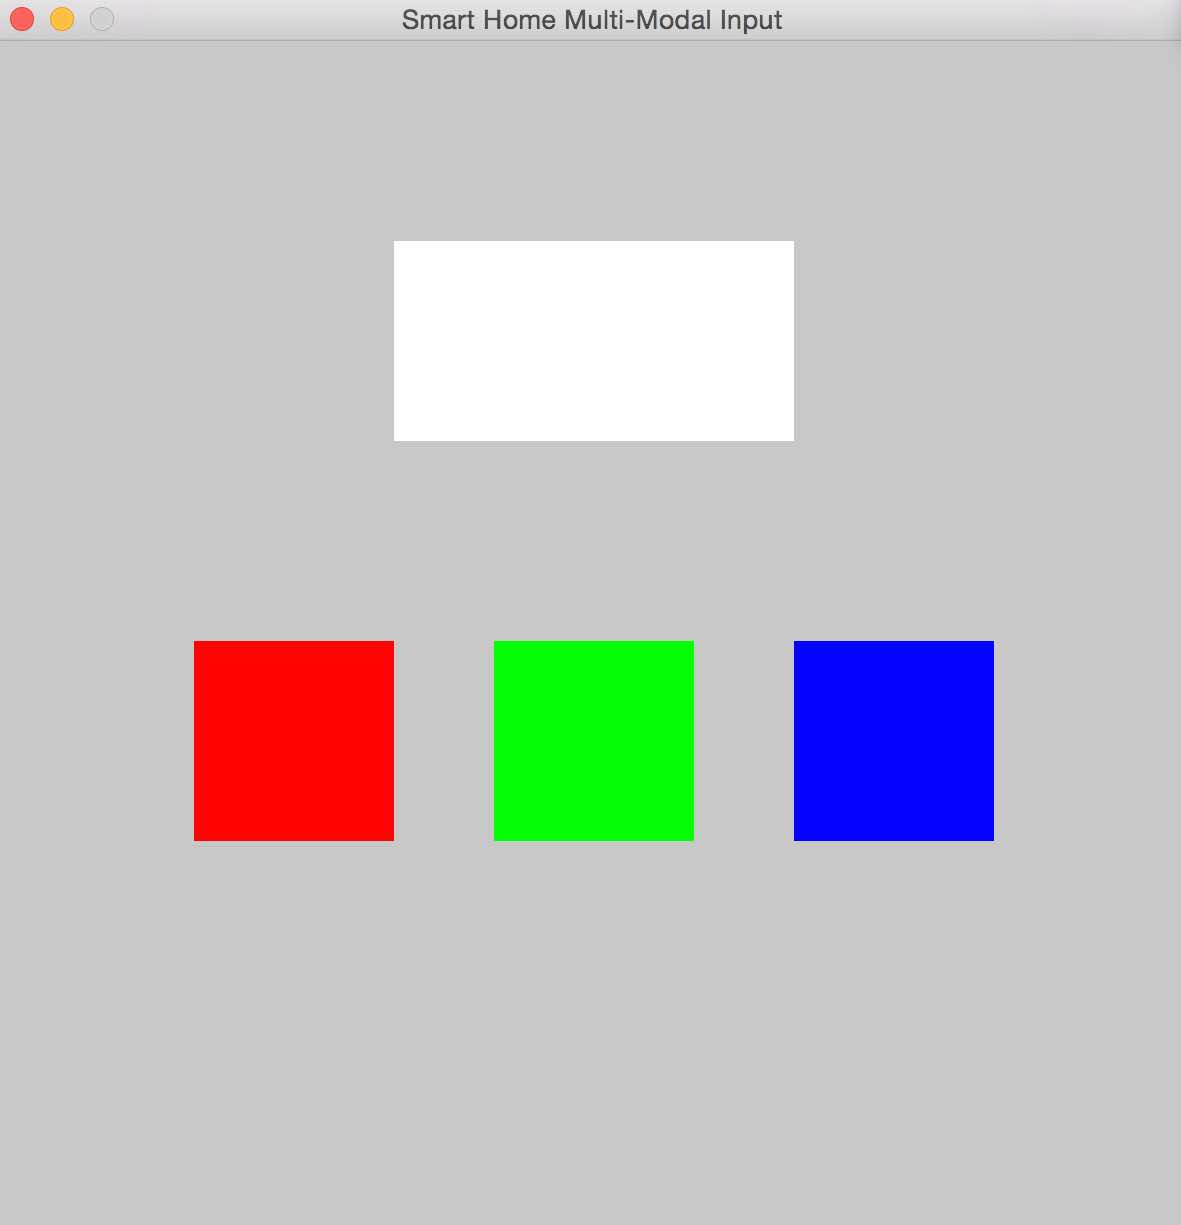
\includegraphics[width=3cm, height=3cm]{fig/color-3}
\caption{}
\label{fig:color-3}
\end{subfigure}
\caption{Illustrasjon lys og fargenivå.}
\label{fig:color}
\end{figure}

\begin{figure}[h]
\centering
\begin{subfigure}{0.23\textwidth}
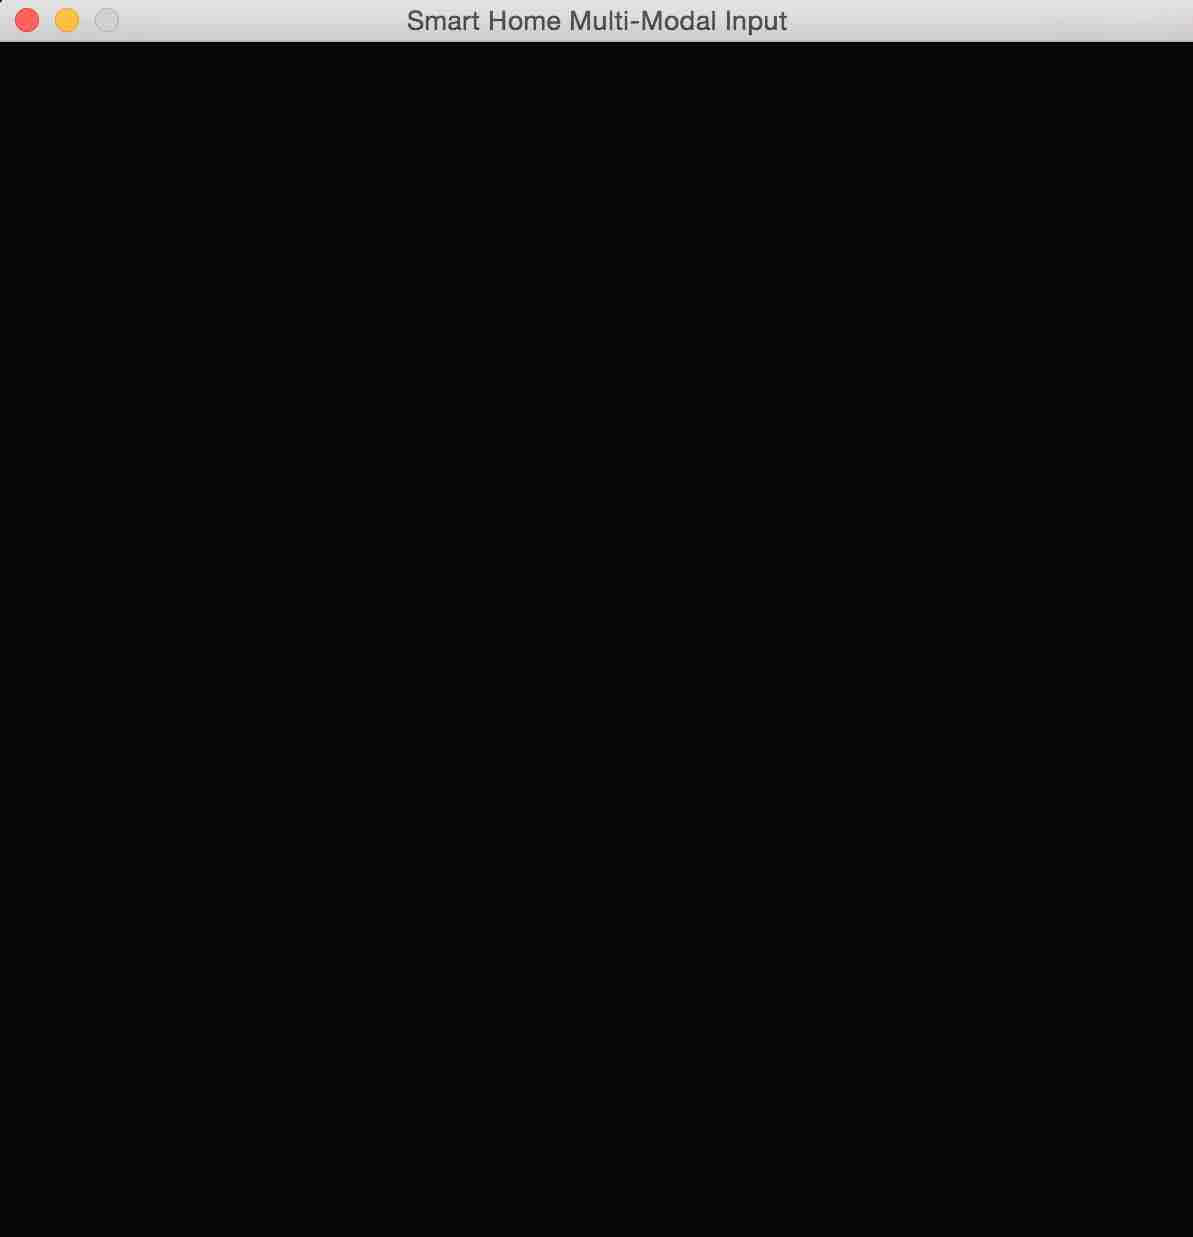
\includegraphics[width=3cm, height=3cm]{fig/light-1}
\caption{}
\label{fig:light-1}
\end{subfigure}
\begin{subfigure}{0.23\textwidth}
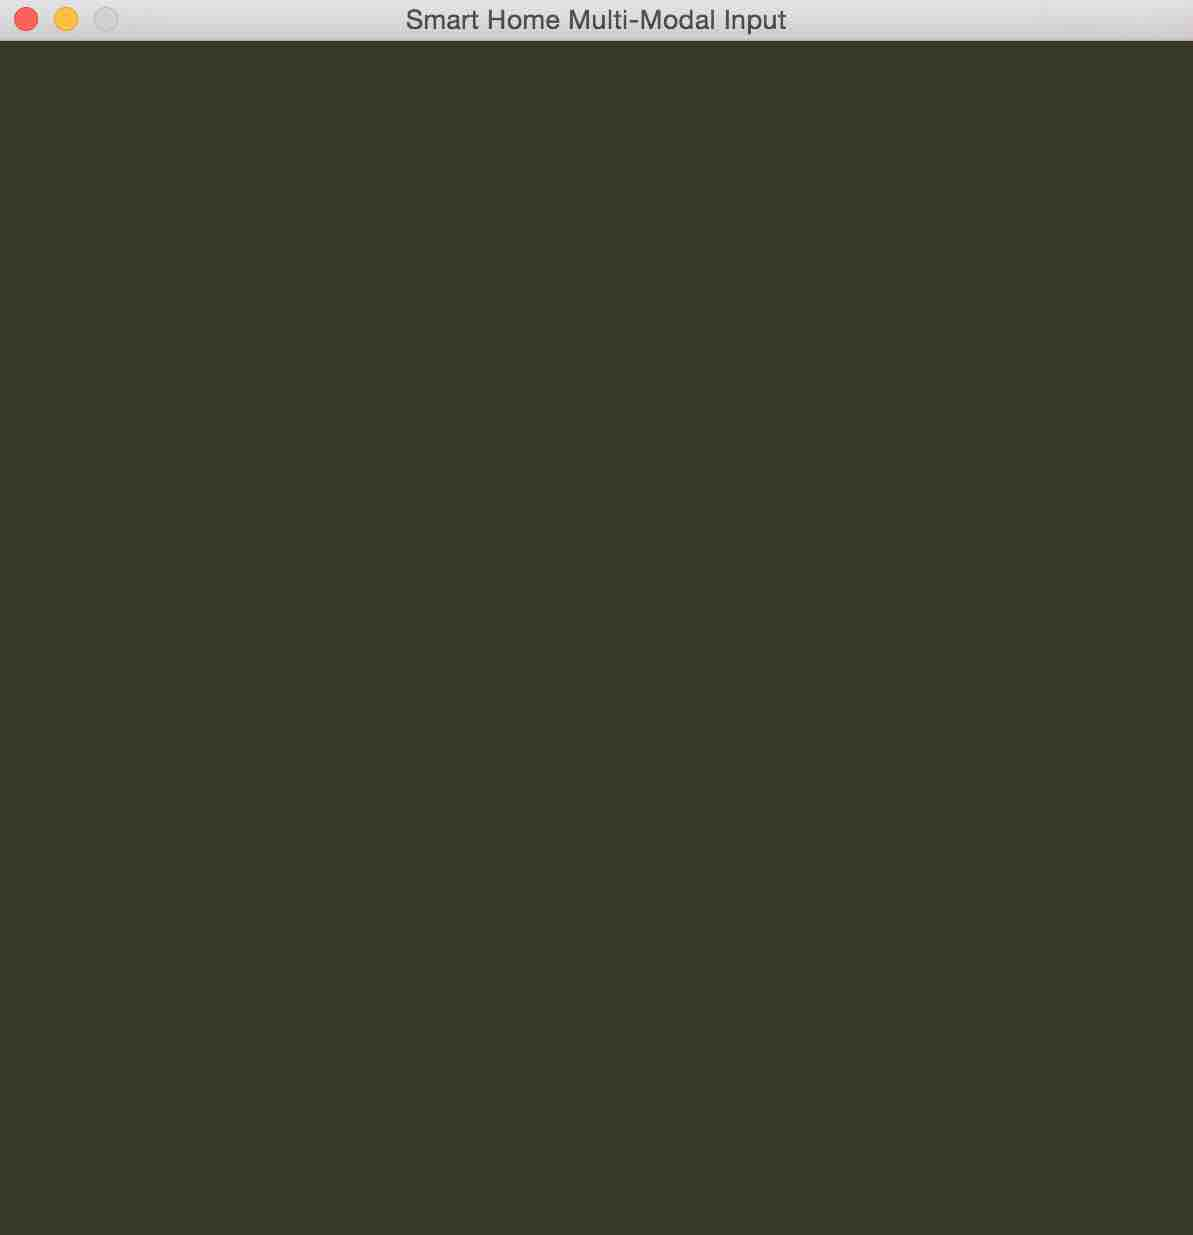
\includegraphics[width=3cm, height=3cm]{fig/light-2}
\caption{}
\label{fig:light-2}
\end{subfigure}
\begin{subfigure}{0.23\textwidth}
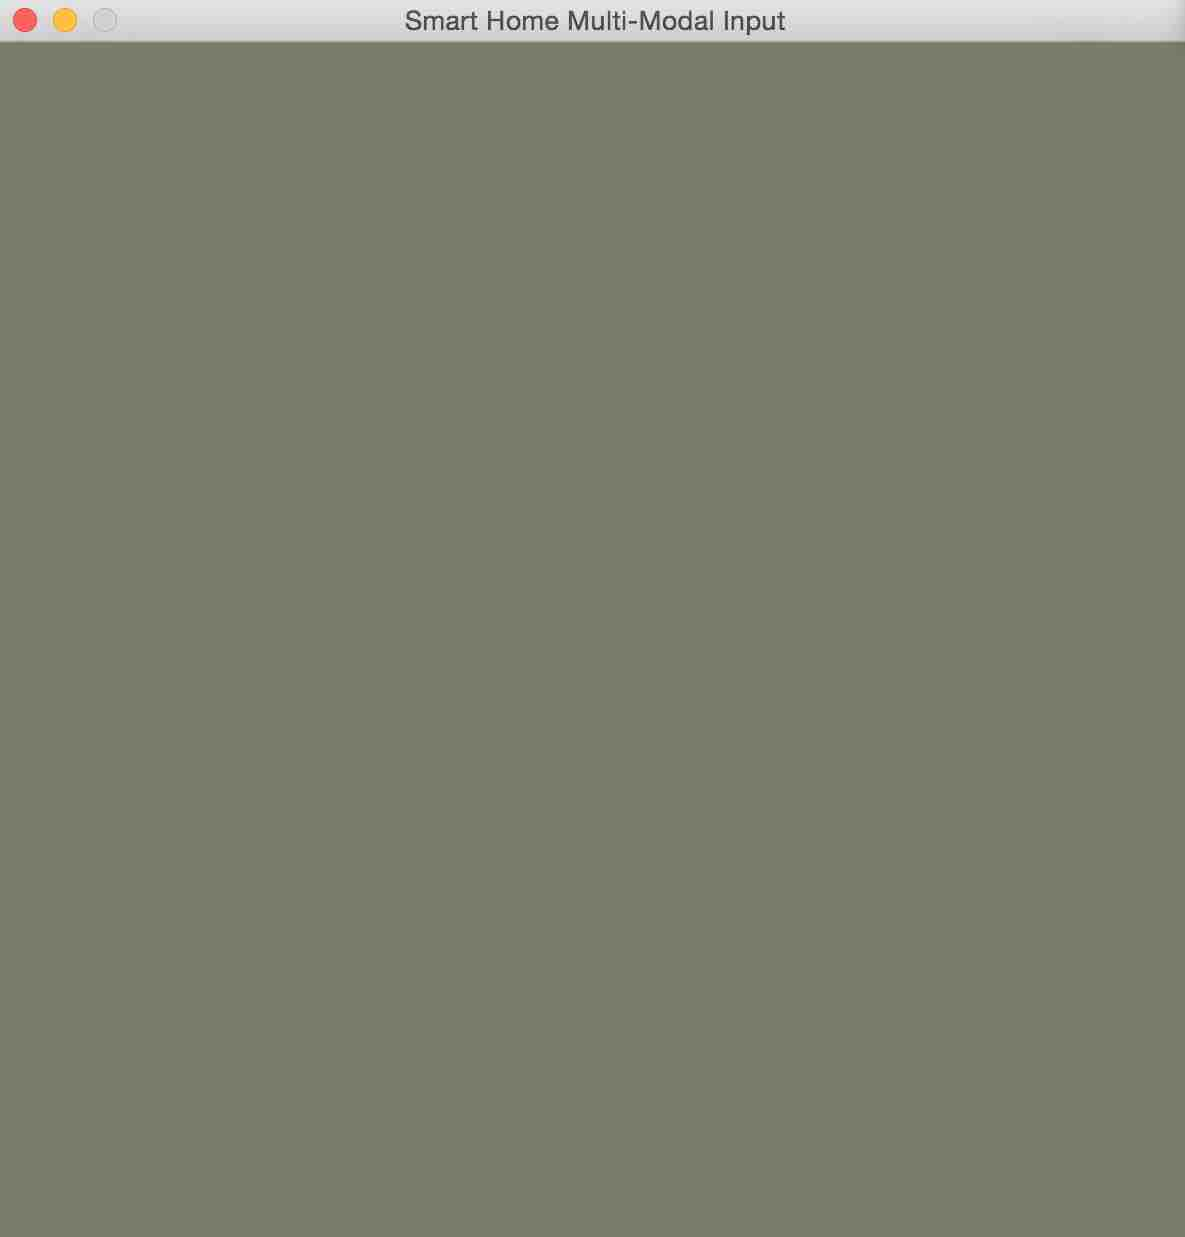
\includegraphics[width=3cm, height=3cm]{fig/light-3}
\caption{}
\label{fig:light-3}
\end{subfigure}
\begin{subfigure}{0.23\textwidth}
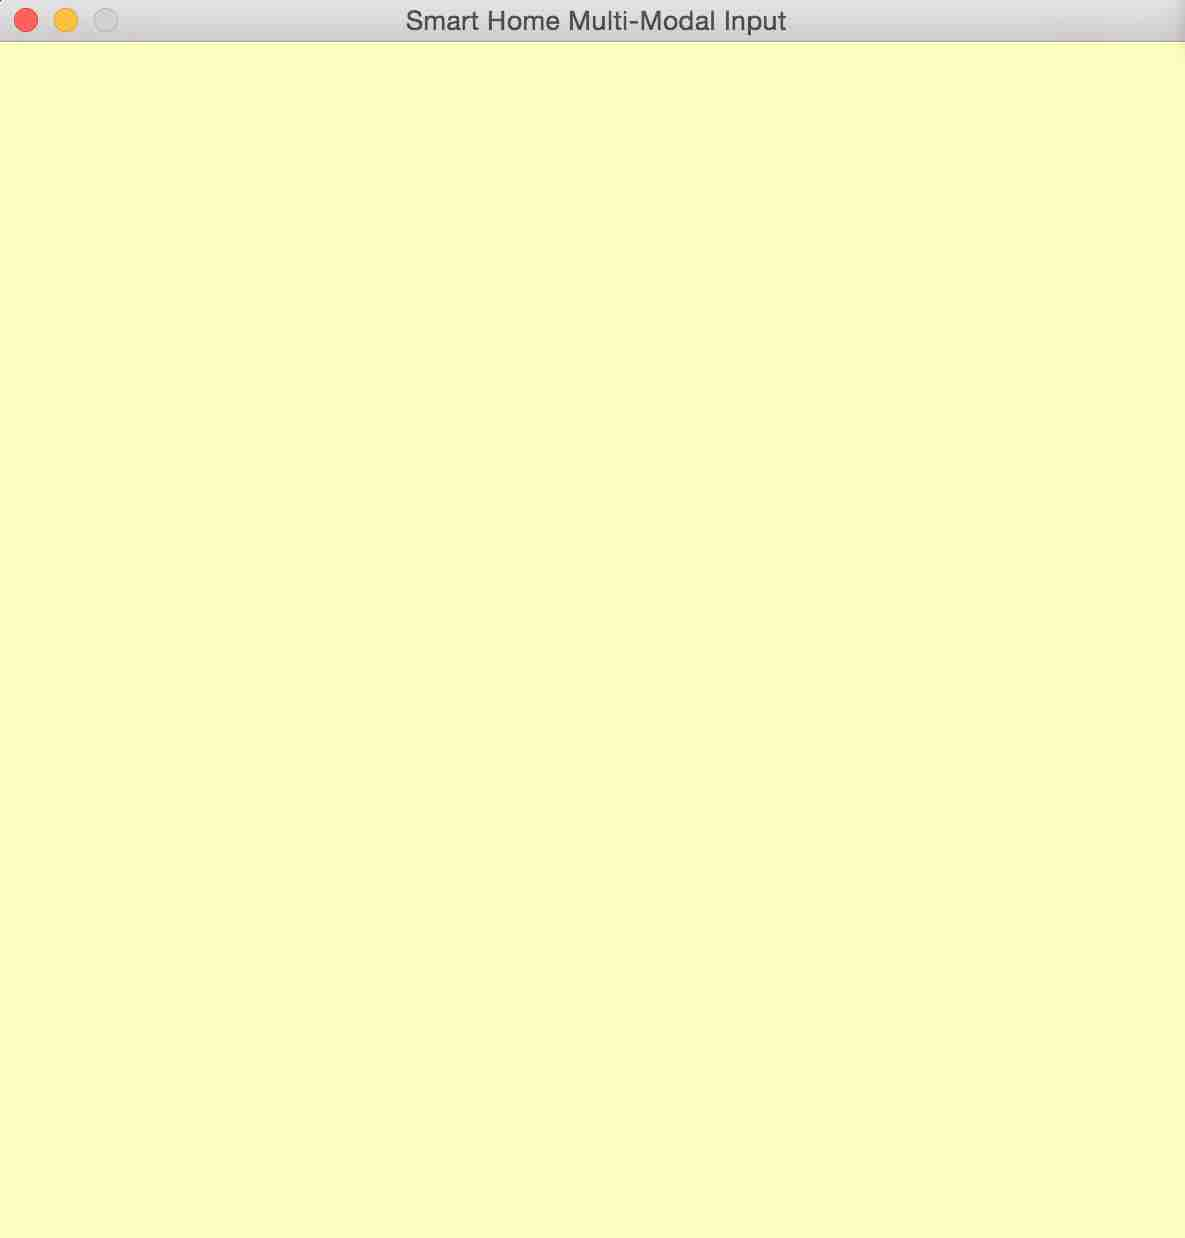
\includegraphics[width=3cm, height=3cm]{fig/light-4}
\caption{}
\label{fig:light-4}
\end{subfigure}
\begin{subfigure}{0.23\textwidth}
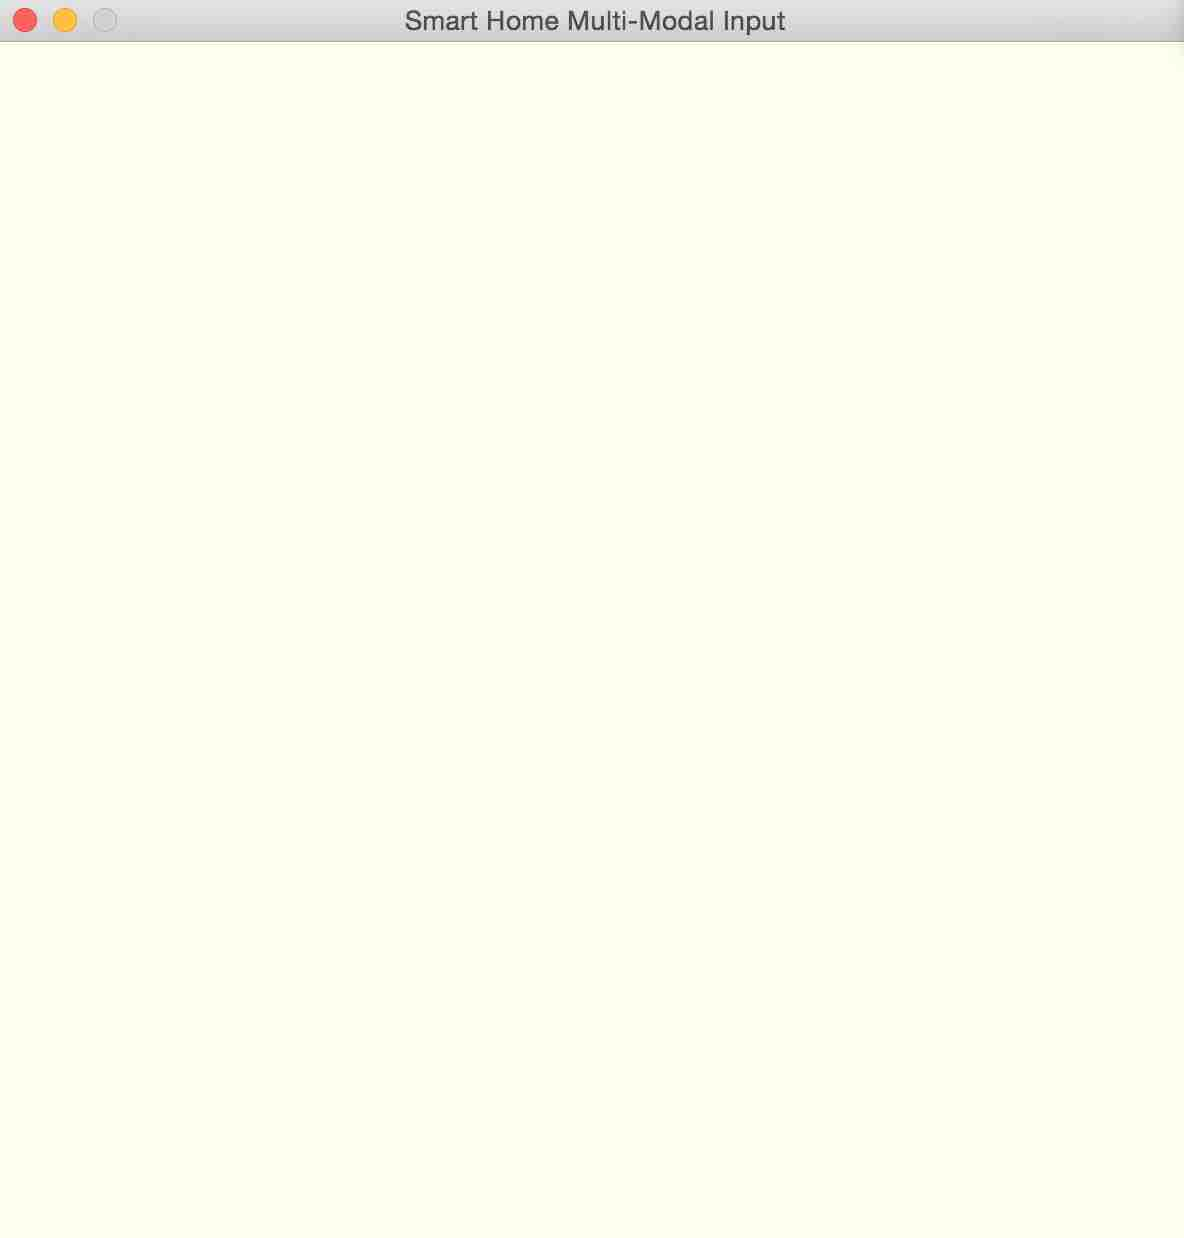
\includegraphics[width=3cm, height=3cm]{fig/light-5}
\caption{}
\label{fig:light-5}
\end{subfigure}
\caption{Illustrasjon dimmeeffekt.}
\label{fig:light}
\end{figure}

\subsubsection{Kontekstdrevet brukergrensesnitt}
{\color{red}Hvordan ble eksperimentet utført?}
Informasjonsprogramvare er ikke en maskin, men et medium for visuell kommunikasjon.

Design av programvare for informasjon burde tilnærmes som grafisk design. Utseende og hvordan informasjon presenteres bør være i fokus. Hva er den relevante informasjonen? Hva vil brukeren vite? Hvordan kan data vises på den mest effektiv måten? Hvordan kan teknikker fra grafisk design anvendes for å lede brukerens blikk mot løsningen? Brukeren bruker programvaren for å lære og han lærer ved å se på programvaren.

Grafisk design er kusten å formidle en beskjed på en to-dimensjonell overflate. Mest relevant til programvare er det Edward Tufte kaller informasjonsdesign, -bruken av bilder for å uttrykke informasjon av interesse for brukeren \citet{tufte01}. En god grafisk designer forstår hvordan informasjon kan posisjoneres på en side slik at leseren kan få svar på spørsmål, gjøre sammenligninger og trekke slutninger. Når programvareutvikleren definerer en visuell representasjon i programmet sitt, utføres grafisk design, nettopp fordi det handler om å definere og posisjonere bildene brukeren skal forstå.

En veldesignet informasjonsgrafikk kan nærmest nøde tilskueren til å stille og svare spørsmål, gjøre sammenligninger og dra slutninger. Dette oppnås ved å utnytte øyets egenskaper. Vi kan raskt og uanstrengt skifte blikket. Vi kan håndtere store mengder visuell data og kan gjenkjenne mønstre og sammenhenger. Vi har også evnen til å skumme en hel side, eller til fokusere på den minste detalj.

Edward Tufte's første regel for statistisk grafisk design: "framfor alt, vis dataene" \citet{tufte01}.

Spørsmål brukeren har om det smarte hjemmet sitt:
\begin{itemize}
\item Hvor lenge er det til vaskeprogrammet er ferdig?
\item Hva er temperaturen i stua nå?
\item Hvor mye strøm brukte vi forrige måned?
\item Trenger jeg å handle inn matvarer?
\item Står det på unødvendig lys og varme i rom vi sjeldent bruker?
\end{itemize}

Hvordan kan disse spørsmålene best besvares?

Hva slags funksjonalitet skal programvaren ha? Å klikke på en lysbryter bør naturligvis skru av eller på lyset. Å klikke på et kjøleskap eller vaskemaskin bør enten skru av og på eller gi mer informasjon om disse apparatene.

Som regel når en person bruker programvare er det ikke for å skape noe, men for å lese, observere, utforske og lære. Folk er ute etter å ordne egne tanker. Datamaskinen er et medium for å spørre spørsmål, gjøre sammenligninger og dra konklusjoner. Det aller meste av programvare er altså \emph{informasjonsprogramvare}. 


Eksempel på typisk brukergrensesnitt:
Dette er ikke en liste over rommene i huset. Det er en informasjonsgrafikk. Den skal benyttes for å lære. Så hvorfor viser vi ikke mer av den tilgjengelige informasjonen?{\color{red}Hvordan data fra det smarte hjemmet er svært rik: sensorer etc..}

Like viktig som hva slags data som vises er hvor dataene vises. Grafikkelementer kan plasseres på bestemte steder for å utnytte vår romforståelse. Desverre er eksisterende programvare for smarte hjem presentert for å maksimere estetikk, ikke for å poengtere og framheve sammenhenger i dataene. {\color{red}Hvordan data om smarte hjem naturlig passer å vise som et kart..}

Kontekst
Datamaskiner kan forstå konteksten rundt hvilke data som trengs, fjerne irrelevant data og generere grafikk som håndterer de nødvendig behovene i øyeblikket.

Design av informasjonsprogramvare er design av kontekst-sensitiv informasjonsgrafikk.

All informasjonsprogramvare består av kontekst-sensitiv grafikk. Tradisjonelt er konteksten definert av brukerinteraksjon. Søkeord og valg i menyer gir programvaren informasjon om hva som er viktig og gir den muligheten til å presentere relevante resultater.

Generelt kan programvare tillegne kontekstinformasjon gjennom tre kanaler:
\begin{itemize}
\item sensorinformasjon fra det fysiske miljøet
\item historie over tidligere valg
\item interaksjon med brukeren
\end{itemize}

Kontekst
Tid, er en av fundamentale dimensjonene som vi organiserer livene våre rundt, og "nå" er det viktigste. Brukere er som regel er ute etter informasjon "nå" eller "snart". Heldigvis vet alle datamaskiner når "nå" er.

Geografisk posisjon. "Her" er viktigst når det gjelder posisjon. Dette kan være litt vanskeligere å bestemme enn tid. Heldigvis har alle smarttelefoner GPS-mottakere. Det finnes også systemer som utvikles for å finne brukeres posisjon innendørs {\color{red}ref MazeMap?}.

Fysisk miljø. Dersom man har tid og posisjon er det for eksempel en smal sak å hente informasjon om været. Det smarte hjemmet vil være fylt til randen av sensorer og informasjon fra det fysiske miljøet blir den viktigste kontekstinformasjonen.

Annen programvare. Dersom brukeren har åpne andre faner eller andre programmer kjørende på maskina kan det forstås hva brukeren er ute etter. {\color{red}leser oppskrift -> info om matvarer som mangler}

Programvare kan bruke historie til å forstå det nåværende tidspunktet. Den nåværende konteksten, eller i det minste en god tilnærming, kan bli gjettet basert på en historie av tidligere miljøer og interaksjoner.

Å gjette basert på den siste kjente verdien, er den enkleste formen for gjetning. Her gjetter programvaren den nåværende konteksten til å være den samme som den forrige. Dette er rimelig i mange situasjoner der brukerens kontekst er nokså statisk og forandrer seg lite over et kort tidsrom. For eksempel, hvis brukeren i går foretrakk å se på en grafisk representasjon av hele huset, er det samme brukeren sannsynligvis interessert i å se det samme den neste dagen. Det ville ikke vært rimelig å neste dag vise informasjon om energiforbruket i huset. Hvis lite, eller ingenting er forandrert bør programvaren vise den samme informasjonen som var foretrukket sist. Den bør vises med en gang og den bør vises uten å spørre om ekstra detaljer.

En enkel tilnærming til læring er å oppdage en felles egenskap mellom foreliggende kontekster, og snevre inn den nåværende konteksten i denne egenskapens retning. Generelt er problemet å forstå et mønster som forklarer brukerens interesser, som en funksjon av miljøet, og så følge mønsteret til å klassifisere det nåværende miljøet. La oss for eksempel si at en bruker benytter programvaren for det smarte hjemmet til å lete fram informasjon om været hver morgen, og bruker den samme programvaren til å se at lys er skrudd av og dørene låst ved sengetid om kvelden. Dersom programvaren kan oppdage og modellere dette mønsteret kan den vise den passende informasjonen til hvert tidspunkt uten at brukeren trenger å be om det. Når brukeren ser på om morgenen vises værmeldingen og ved sengetid vises informasjon om lys og dører.

Programvare for informasjon etterligner opplevelsen av å lese, ikke å jobbe. Det brukes for å oppnå en forståelse og for å konstruere en mental modell. Brukeren må altså lytte til programvaren og tenke på hva den sier. Enhver manipulering foregår i brukerens hode. Den eneste grunnen til å interagere er dermed å eksplisitt gi ekstra kontekstinformasjon som programvaren ikke selv kan finne ut av. Dette indikerer subsettet av informasjon som er relevant. For programvare for informasjon er interaksjon å navigere i dataene.

For programvare for informasjon er all interaksjon å spesifisere kontekst. Hver interaksjon bør resultere i en forståelig forandring i kontekst-sensitiv informasjonsgrafikk. Ved å gi direkte tilbakemelding reduserer mengden manipulasjon brukeren må utføre for å få et tilstrekkelig syn på dataene.

Kontekst kan forstås fra brukerinteraksjon, men kun som en siste utvei. Den beste måten å minimere eller fjerne interaksjon er gjennom informasjonsrik grafisk design, som bruker miljøet og historie. Gjenværende interaksjon kan løses med grafisk manipulasjon, relativ navigasjon og en tett feedback-loop.

Dersom programvaren kan forstå så mye som mulig fra historie og fra miljøet bør den i det minste klare å produsere et rimelig utgangspunkt. Mesteparten av brukerens interaksjon blir derfra å korrigere eller bekrefte programmets gjetninger. Denne tilnærmingen er som regel enklere enn å skape all kontekst fra begynnelsen av.

Dersom en bruker trykker på en knapp og ingenting skjer, er det vanskelig å forstå om handlingen utførte noe som helst. Brukeren kan ikke evaluere en respons og la den lede til en ny handling. Spesielt for informasjonsprogramvare danner all interaksjon kontekst. Dermed bør enhver interaksjon skape en merkbar forvandling i grafikken. Å gi direkte tilbakemelding reduserer mengden manipulasjon brukeren må utføre for å nå en tilstand der den ønskede informasjonen er tilgjengelig.

I stedet for å vite navnet på en gjenstand eller et rom kan brukeren i praksis peke på kartet og si "der!". Feedback-loopen er svært tett: dersom brukeren pekte på en del som kan interageres med oppdateres viewet umiddelbart. 

Det er noen forsøk på å bruke farger symbolsk i grafikken. Elementer med klare rødfarger er avslått eller låst. Elementer med klare grønnfarger er på eller åpne. Kjøleskapet er i en klar farge for å indikere at den kan interageres med. Ellers er elementene som utgjør bakgrunnen i grafikken i grå, utvaskede eller sjenerte farger.

Hver gang brukeren viser interesse i en gitt skjermvisning blir det lagret i en historie med tidspunktet. Brukeren viser interesse ved å trykke på et element som forandrer visning eller på en av de tilgjengelige knappene.

As with the map, once the information graphic is established, manipulation can be incorporated.
Når dette kartet over huset er etablert som en informasjonsgrafikk, kan manipulasjon bli tilgjengeliggjort.

Brukeren ser alltid at programmet viser informasjonen om huset. Dersom det som vises ikke er konfigurasjonen brukeren ønsker kan det forandres på stedet. Det er ingen "OK", "submit" eller "apply"-knapp. Kartet viser alltid den nåværende tilstanden til hjemmet.




\subsection{Resultater}
\subsubsection{Gestegjenkjennelse gjennom fotodioder}
{\color{red}Hva var resultatet av eksperimentet?}

\begin{table}[h!]
\centering
\begin{tabular}{|| c c c c ||}
\hline
\% Korrekt klassifisering & Algoritme & Antall gester & Treningseksempler/gets \\ [0.5ex] 
 \hline\hline
 96,0 & SVM m/libsvm & 10 & 50 \\ 
 \hline
 95,8 & SVM m/liblinear & 10 & 50 \\
 \hline
 94,048 & Logistisk regresjon & 10 & 50 \\ [1ex]
 \hline
\end{tabular}
\caption{Gjennomsnittsresultater for klassifisering av 10 gester.}
\label{table:results}
\end{table}

Modellene er trent og testet 100 ganger med tilfeldige utgangspunkt.

\begin{figure}[h!]
\centering
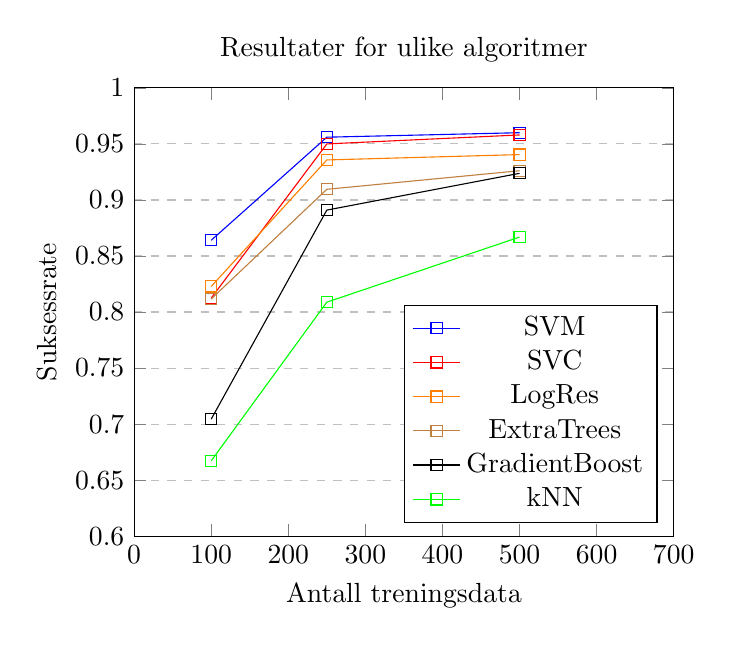
\begin{tikzpicture}
\begin{axis}[
    title={Resultater for ulike algoritmer},
    xlabel={Antall treningsdata},
    ylabel={Suksessrate},
    xmin=0, xmax=700,
    ymin=0.6, ymax=1.0,
    xtick={0,100,200,300,400,500,600,700},
    ytick={0.6,0.65,0.7,0.75,0.8,0.85,0.9,0.95,1.0},
    legend pos=south east,
    ymajorgrids=true,
    grid style=dashed,
]
\addplot[
    color=blue,
    mark=square,
    ]
    coordinates {
    (100,0.864)(250,0.956)(500,0.96)
    };
\addplot[
    color=red,
    mark=square,
    ]
    coordinates {
    (100,0.8124)(250,0.95)(500,0.958)
    };
\addplot[
    color=orange,
    mark=square,
    ]
    coordinates {
    (100,0.8228)(250,0.9357)(500,0.94048)
    };
\addplot[
    color=brown,
    mark=square,
    ]
    coordinates {
    (100,0.8116)(250,0.9095)(500,0.92608)
    };
\addplot[
    color=black,
    mark=square,
    ]
    coordinates {
    (100,0.7044)(250,0.89095)(500,0.92376)
    };
\addplot[
    color=green,
    mark=square,
    ]
    coordinates {
    (100,0.6672)(250,0.8088)(500,0.86688)
    };
    
    \legend{SVM,SVC,LogRes,ExtraTrees,GradientBoost,kNN}
\end{axis}
\end{tikzpicture}
\label{figure:resultsgraf}
\caption{Resultatsutvikling for et utvalg algoritmer.}
\end{figure}

Både logistisk regresjon og støttevektormaskin ga svært lovende resultater, som vist i tabell \ref{table:results}. 96\% er en meget høy suksessrate og viser hvor godt enkle, lineære modeller kan skille på denne typen data. Det ble så interessant å spørre seg om dette resultatet kunne blitt enda høyere. Jeg ønsket ikke å bruke mer tid på å lage flere treningseksempler, så i stedet utførte jeg treningen på nytt med færre treningseksempler, i håp om å kunne se en utviklingstrend. Det samme eksperimentet ble utført med en femtedel og halvparten av dataene for å danne et bilde av sammenhengen mellom forbedring i suksessrate og antall treningseksempler. Figur \ref{figure:resultsgraf} viser resultatene for 100, 250 og 500 treningseksempler. Ettersom biblioteket jeg benyttet for å implementere algoritmene tilbyr en rekke andre algoritmer forsøkte jeg noen andre tilnærminger enn lineære modeller og inkluderte dem også.

I figur \ref{figure:resultsgraf} kan vi se at SVM-ene er i nærheten av 95\% allerede etter 250 treningseksempler og at de kun øker minimalt med 250 ekstra tilfeller. Dette tyder på at det trengs et stort antall ekstra treningseksempler for at algoritmene skal krype betydelig nærmere 100\%. De mer kompliserte algoritmene ExtraTrees og GradientBoost benytter seg av flere algoritmer under panelet og kombinerer disse. Det kan se ut som om spesielt GradientBoost kan fortsette å øke suksessraten betydelig med mer trening, men det er tvilsomt om den noen gang passerer SVM. Til sist nevnes k-nærmeste nabo (kNN), som begynner svakest av de utprøvde algoritmene, men fremdeles har en sterk vekst mellom 250 og 500 tilfeller. Det hadde vært interessant å se utviklingen videre for denne enkle algoritmen.

Dette prosjektet har argumentert for at gester kan være en aktuell interaksjonsform i hjemmet, spesielt som en erstatning til store knappepaneler og desentralisert styringskontroll. Det har også vist at maskinlæring kan benyttes for å gi enkle sensorer en svært god forståelse av gester. Med en suksessrate på over 95\% i klassifiseringen av 10 ulike gester er denne teknikken svært interessant. Og med en suksessrate på over 85\% allerede etter kun 10 treningseksempler på hver gest, kan man forestille seg at brukere selv kan sette av 10 minutter til å trene et helt nytt og utrent system til å forstå sine egne gester. I et produkt kunne det vært aktuelt å tilby online-læring gjennom systemets levetid. Man kan med andre ord la systemet lære etter hvert som brukeren benytter systemet. Dette vil nødvendigvis kreve at brukeren har en mulighet til å gi tilbakemelding på når systemet gjettet riktig gest og når det gjettet feil.

\subsubsection{Multimodal interaksjon gjennom tale og gester}
{\color{red}Hva var resultatet av eksperimentet?}


\subsubsection{Kombinasjoner}
{\color{red}Hva var resultatet av eksperimentet?}

\begin{table}[h!]
\centering
\begin{tabular}{|| c c c c ||}
\hline
\% Korrekt klassifisering & Algoritme & Antall gester & Treningseksempler/gest \\ [0.5ex] 
 \hline\hline
 94,12 & SVM m/liblinear & 10 & 10 \\ 
 \hline
 92,48 & Logistisk regresjon & 10 & 10 \\ [1ex]
 \hline
 92,4 & SVM m/libsvm & 10 & 10 \\
 \hline
\end{tabular}
\caption{Gjennomsnittsresultater for klassifisering av de samme 10 gestene fra eksperiment 1.}
\label{table:results-foursensors}
\end{table}

Langt bedre resultater enn 10 samples av hver over en sensor (.86 .82 .81). Liblinear-algoritmen og logistisk regresjon slår libsvm.  Modellene er trent og testet 100 ganger med tilfeldige utgangspunkt.

\begin{table}[h!]
\centering
\begin{tabular}{|| c c c c ||}
\hline
\% Korrekt klassifisering & Algoritme & Antall gester & Treningseksempler/gest\\ [0.5ex] 
 \hline\hline
 94,124 & SVM m/libsvm & 42 & 10 \\ 
 \hline
 93,333 & SVM m/liblinear & 42 & 10 \\
 \hline
 92,59 & Logistisk regresjon & 42 & 10 \\ [1ex]
 \hline
\end{tabular}
\caption{Gjennomsnittsresultater for klassifisering av 42 gester.}
\label{table:results-foursensors}
\end{table}

Med kun 10 treningseksempler av hver av de 42 gestene oppnås en suksessrate på 94\%. Modellene er trent og testet 100 ganger med tilfeldige utgangspunkt.

\subsubsection{Kontekstdrevet brukergrensesnitt}
{\color{red}Hva var resultatet av eksperimentet?}
